
\documentclass{article} % For LaTeX2e
\usepackage{iclr2027_conference,times}

% Optional math commands from https://github.com/goodfeli/dlbook_notation.
\input{math_commands.tex}

\usepackage{hyperref}
\usepackage{url}
\usepackage{amsmath,amssymb}
\usepackage{booktabs}
\usepackage{graphicx}
\usepackage{array}
\usepackage{algorithm}
\usepackage{algpseudocode}

\DeclareMathOperator*{\argmaxop}{arg\,max}
\DeclareMathOperator{\Dec}{Dec}
\DeclareMathOperator{\sgop}{sg}
\newcommand{\fitbox}[1]{\resizebox{\ifdim\width>\linewidth\linewidth\else\width\fi}{!}{#1}}

\title{Scored Consistency Distillation of SD3.5-Medium\\with a Decode-Free Photographic Reward}

\author{Anonymous Author(s) \\ Affiliation \\ Address \\ \texttt{email}}

%\iclrfinalcopy % Uncomment for camera-ready version, but NOT for submission.
\begin{document}

\maketitle

\section{Method}
\label{sec:method}

We distil SD3.5-Medium, a 2.5B-parameter rectified-flow transformer, into a 4-step student. The
method has two parts. First, for every training caption the frozen teacher produces several
candidate generations, and a scorer that reads a reference photograph of the caption picks one of
them; the student is trained only on the picked trajectory. Second, a differentiable, decode-free
photographic reward term pulls the student's own predictions toward the same photograph during
training, computed by a small trained network rather than by decoding through the VAE. Both parts
use the same underlying quantity, the DINOv2 similarity of an image to the photograph the caption
describes, and neither reads the caption text or any language model.

\subsection{Preliminaries: rectified-flow distillation}
\label{sec:prelim}
The teacher is a rectified-flow model with frozen weights $\theta_T$, operating in the $D$-dimensional
latent space of a frozen VAE ($D{=}65{,}536$ at $512{\times}512$ pixels: a $16{\times}64{\times}64$
latent). A clean latent $x_0\in\mathbb R^D$ and
Gaussian noise $\varepsilon\sim\mathcal N(0,I)$ define a straight path $z_\sigma=(1-\sigma)x_0+\sigma\varepsilon$,
$\sigma\in[0,1]$, and the network predicts the velocity $v=\varepsilon-x_0$ conditioned on the
caption $c$. Sampling is Euler integration on a $\sigma$ grid, $z_{k+1}=z_k+(\sigma_{k+1}-\sigma_k)\,v_\theta(z_k,\sigma_k,c)$,
with classifier-free guidance $v^{\mathrm{cfg}}=v_\theta(z,\sigma,\varnothing)+w\big(v_\theta(z,\sigma,c)-v_\theta(z,\sigma,\varnothing)\big)$
at $w=7$ for the teacher. The student $v_\theta$ is a full copy of the same transformer, initialised
from $\theta_T$, and is the only network that trains; the teacher, the text encoders and the VAE
decoder $\Dec$ stay frozen throughout. There is no momentum target, no exponential moving average
and no stop-gradient copy of the student anywhere in the recipe: every training target below is a
deterministic function of the frozen teacher.

Consistency distillation trains the student to jump directly to the clean-latent estimate that the
teacher reaches only after several further steps, so that a 4-step Euler rollout of the student
reproduces an 8-step teacher trajectory. This is the sole mechanism that turns an 8-step teacher
into a 4-step student; nothing below changes it. What varies is which trajectory the student is
trained on, and what, besides matching that trajectory, the training loss asks the student's own
predictions to do.

\subsection{Candidate generation and photographic scoring}
\label{sec:selection}
For every training caption $c$ with reference photograph $x^{\mathrm{ref}}$ (its COCO source image),
we draw $N=4$ candidate teacher trajectories from four independent seeds and score each one against
the photograph.

\paragraph{Candidates.} Candidate $j$ uses Gaussian noise $\varepsilon^{(j)}$ seeded deterministically
from the caption index, and is an 8-step Euler rollout of the teacher at guidance $w=7$:
\begin{equation}
\varepsilon^{(j)}\sim\mathcal N(0,I)\ \text{(seeded by caption and $j$)},\qquad
z^{(j)}_0,\dots,z^{(j)}_8=\mathrm{Euler}_{K=8}\big(\varepsilon^{(j)};v_T^{\mathrm{cfg}},c\big).
\end{equation}
Only the seed, not the trajectory, needs to be stored: any candidate can be re-rolled exactly from
its seed whenever it is needed again, at scoring time and later at training time.

\paragraph{Scoring.} Each candidate is decoded, $I_j=\Dec(z^{(j)}_8)$, and embedded with a frozen
DINOv2-B vision transformer. We drop the CLS token, mean-pool the $P{=}256$ patch tokens and
$\ell_2$-normalise:
\begin{equation}
u(I)=\frac{\frac1P\sum_{p=1}^{P}h_p(I)}{\big\lVert\frac1P\sum_{p=1}^{P}h_p(I)\big\rVert},\qquad
S_j=\big\langle u(I_j),\,u(x^{\mathrm{ref}})\big\rangle .
\label{eq:score}
\end{equation}
$u(x^{\mathrm{ref}})$ is computed once per caption. This scorer needs no caption text, no VLM and no
learned preference model: it is a fixed, off-the-shelf self-supervised image encoder, applied
identically to a generated candidate and to a real photograph.

\paragraph{Selection.} We select the best candidate by hard argmax over the score,
\begin{equation}
j^\star=\argmaxop_{j\in\{1,\dots,N\}}S_j ,
\label{eq:argmax}
\end{equation}
and every subsequent training visit of caption $c$ trains only on trajectory $j^\star$. Selection is
computed once, offline, before training starts, and is never revisited: no gradient flows through
the scorer, and the training loop simply re-rolls trajectory $j^\star$ from its stored seed. A random
baseline replaces $j^\star$ with a uniform draw over $\{1,\dots,N\}$, stored so that every training
seed sees the same draw; this isolates the effect of \emph{which} trajectory a caption trains on
from everything else in the recipe.

\subsection{Consistency distillation loss}
\label{sec:cd}
Let $z_0,\dots,z_8$ be the selected teacher trajectory. Training supervises a window of states
$\mathcal K=\{3,4,5,6,7\}$ on the 8-step grid. For $k\in\mathcal K$, the teacher's realised chord
across its own step and the clean-latent estimate it implies are
\begin{equation}
\bar v_k=\frac{z_{k+1}-z_k}{\sigma_{k+1}-\sigma_k},\qquad
\tilde x_0^{(k)}=z_k-\sigma_k\,\bar v_k ,
\end{equation}
which is exact algebra for a straight path. The student is placed at a \emph{noisier} state than the
one the target was read from: for each $k$ we draw $\Delta_k\sim\mathcal U\{1,2,3\}$ independently and
afresh on every visit, set $s=k-\Delta_k$, and the student forms its own clean-latent estimate with a
single conditional forward pass and no guidance,
\begin{equation}
\hat x_0^{(s)}=z_s-\sigma_s\,v_\theta(z_s,\sigma_s,c).
\end{equation}
The consistency loss is a pseudo-Huber distance in $x_0$-space, averaged over the window:
\begin{equation}
\ell_c(\theta)=\frac{1}{|\mathcal K|}\sum_{k\in\mathcal K}\rho\Big(\hat x_0^{(k-\Delta_k)}-\sgop\big[\tilde x_0^{(k)}\big]\Big),
\qquad \rho(u)=\sqrt{\lVert u\rVert_2^2+c_h^2}-c_h ,
\label{eq:cdloss}
\end{equation}
with $\sgop[\cdot]$ a stop-gradient and $c_h=0.00054\sqrt D\approx0.138$ a small constant scaled to
the latent dimensionality (the pseudo-Huber loss behaves like an $\ell_2$ distance below $c_h$ and
like an $\ell_1$ distance above it).
Because the student is trained with a single conditional pass against $w{=}7$ teacher trajectories,
guidance is absorbed into its prediction: the student is sampled at $w{=}1$, with no classifier-free
guidance at inference.

\subsection{A decode-free photographic reward}
\label{sec:reward}
Selection alone only changes which of the teacher's four trajectories the student is trained on; it
never moves the student's own predictions toward the photograph directly. The reward does, and it
does so \emph{without ever decoding a training image}: a small trained network $P_\phi$ maps a
latent directly into the DINOv2 patch-mean space of Section~\ref{sec:selection}, so a reward can be
computed and differentiated on the student's own latent prediction with no VAE decode, no DINOv2
forward pass, and no dependence on either at training time.

\paragraph{Projector network and its offline pretraining.} $P_\phi:\mathbb R^{16\times64\times64}\to\mathbb R^{768}$
is a 6.8M-parameter convolutional encoder (five blocks, channel widths $64,128,256,512,512$, the
last four downsampling by 2, global-average-pooled) followed by a two-layer MLP head
($512{\to}1024{\to}768$) and an $\ell_2$-normalisation. It is pretrained once, offline, on 22,000
captions disjoint from any pool it will later score: for each cached candidate $z_j$ with true
embedding $e_j=u(\Dec(z_j))$ and true score $S_j=\langle e_j,u(x^{\mathrm{ref}})\rangle$,
\begin{equation}
\mathcal L_{\mathrm{pre}}(\phi)=\mathrm{mean}_j\big[1-\langle P_\phi(z_j),e_j\rangle\big]\;+\;\mathrm{KL}\Big(\mathrm{softmax}(S/\tau)\,\big\|\,\mathrm{softmax}(\hat S/\tau)\Big),\qquad \hat S_j=\langle P_\phi(z_j),u(x^{\mathrm{ref}})\rangle,
\label{eq:projpretrain}
\end{equation}
$\tau{=}0.04$, 30 epochs, batch 32 captions (128 candidates), AdamW with a one-cycle schedule
peaking at $3\times10^{-4}$; the first term matches the embedding directly, the second preserves the
within-caption ranking of the four candidates. The pretrained $P_\phi$ is then frozen and used to
compute the training-time reward.

\paragraph{Reward.} On every training update, the student's own clean-latent estimates at the two
least-noisy supervised states are scored by $P_\phi$ directly, with no decode:
\begin{equation}
r_c(\theta;\phi)=\frac12\sum_{i=1}^{2}\big\langle P_\phi\big(\hat x_0^{(s_i)}\big),\,u(x^{\mathrm{ref}})\big\rangle .
\label{eq:reward}
\end{equation}
The full per-caption training objective is
\begin{equation}
\mathcal L(\theta)=\mathbb E_c\big[\ell_c(\theta)\big]\;-\;\lambda\,\mathbb E_c\big[r_c(\theta;\phi)\big] ,
\label{eq:objective}
\end{equation}
combining Equations~\ref{eq:cdloss} and~\ref{eq:reward}, with $\lambda{=}80$ (set, like the exact
reward's weight, so the raw reward gradient starts at about 20\% of the raw consistency gradient's
norm; $P_\phi$'s outputs live on a different scale than the true DINOv2 embeddings, so this weight
is not comparable in magnitude to a decode-based reward's).

\paragraph{Periodic refresh.} $P_\phi$ was pretrained on the teacher's own candidates, not on a
4-step student's evolving predictions, so its accuracy on the distribution it is actually scoring
during training is not guaranteed. To address this, every 100 training updates $P_\phi$ is briefly
unfrozen and fit to the true DINOv2 embedding of the student's own recent predictions (decoded just
for this refresh step, not for the reward itself), together with a replay term on a fresh batch of
the original teacher-candidate data so it does not forget how to rank them:
\begin{equation}
\mathcal L_{\mathrm{refresh}}(\phi)=\mathrm{mean}\big[1-\langle P_\phi(\hat x_0),\,u(\Dec(\hat x_0))\rangle\big]\;+\;\mathcal L_{\mathrm{pre}}(\phi)\ \text{on a replay batch},
\label{eq:refresh}
\end{equation}
16 AdamW steps at learning rate $10^{-4}$ each time, after which $P_\phi$ is frozen again until the
next refresh. This variant -- more refresh steps per event than the default of 4 -- is the
best-scoring configuration of the projector-reward family we tested (Section~\ref{sec:results-align}).

\subsection{Training algorithm}
\label{sec:pseudocode}
Algorithm~\ref{alg:select} chooses one trajectory per caption, once, before training starts, and
still decodes and scores candidates offline -- that part of the pipeline is unchanged. Algorithm~\ref{alg:projpretrain}
pretrains the projector $P_\phi$, once, before any student training. Algorithm~\ref{alg:train} is
the training loop itself: it never decodes a latent to compute the reward, only $P_\phi$ is called,
and every 100 updates $P_\phi$ is briefly refit (lines~\ref{ln:refresh-start}--\ref{ln:refresh-end}).

\begin{algorithm}[t]
\caption{Choose a trajectory for every caption (once, before training)}
\label{alg:select}
\begin{algorithmic}[1]
\Require training captions with reference photographs $x^{\mathrm{ref}}$; frozen teacher $v_T$; frozen decoder $\Dec$; frozen DINOv2 scorer $u(\cdot)$
\For{each training caption $c$}
  \For{$j=1,\dots,N$, with $N{=}4$}
    \State draw noise $\varepsilon^{(j)}\sim\mathcal N(0,I)$ from a seed fixed by $(c,j)$
    \State roll out the teacher for 8 Euler steps at guidance $w{=}7$: $z^{(j)}_0,\dots,z^{(j)}_8=\mathrm{Euler}_8(\varepsilon^{(j)};v_T,c)$
    \State decode and score: $I_j\gets\Dec(z^{(j)}_8)$,\quad $S_j\gets\langle u(I_j),\,u(x^{\mathrm{ref}})\rangle$ \Comment{Equation~\ref{eq:score}}
  \EndFor
  \State $j^\star\gets\argmaxop_j S_j$ \Comment{Equation~\ref{eq:argmax}}
  \State keep only $(c,\ \text{the seed of } j^\star,\ z^{(1)}_8,\dots,z^{(4)}_8,\ e_1,\dots,e_4{=}u(I_1),\dots,u(I_4))$ \Comment{terminal latents + true embeddings kept as pretraining/replay data}
\EndFor
\end{algorithmic}
\end{algorithm}

\begin{algorithm}[t]
\caption{Pretrain the projector $P_\phi$ (once, before any student training)}
\label{alg:projpretrain}
\begin{algorithmic}[1]
\Require 22,000 captions' cached candidates from Algorithm~\ref{alg:select} ($z_j$, true embedding $e_j$, true score $S_j$), disjoint from any pool $P_\phi$ will later score; $\tau{=}0.04$
\State initialise $P_\phi$: 5-block conv encoder (widths 64,128,256,512,512) + MLP head ($512{\to}1024{\to}768$) + $\ell_2$-normalise
\For{30 epochs, batches of 32 captions (128 candidates)}
  \State $\hat e_j\gets P_\phi(z_j)$;\quad $\hat S_j\gets\langle\hat e_j,u(x^{\mathrm{ref}})\rangle$
  \State $\mathcal L_{\mathrm{pre}}\gets\mathrm{mean}_j[1-\langle\hat e_j,e_j\rangle]+\mathrm{KL}\big(\mathrm{softmax}(S/\tau)\,\|\,\mathrm{softmax}(\hat S/\tau)\big)$ \Comment{Equation~\ref{eq:projpretrain}}
  \State AdamW step on $\phi$ (one-cycle schedule, peak lr $3{\times}10^{-4}$)
\EndFor
\State freeze $\phi$; this is the $P_\phi$ used by Algorithm~\ref{alg:train} below
\end{algorithmic}
\end{algorithm}

\begin{algorithm}[t]
\caption{Train the student (one optimiser step; repeat until the schedule ends)}
\label{alg:train}
\begin{algorithmic}[1]
\Require student $v_\theta$ (trainable, initialised from $\theta_T$); frozen teacher $v_T$; frozen decoder $\Dec$; frozen DINOv2 scorer $u(\cdot)$; pretrained projector $P_\phi$ (Algorithm~\ref{alg:projpretrain}); replay buffer of teacher-candidate data (Algorithm~\ref{alg:select}); window $\mathcal K=\{3,\dots,7\}$; reward weight $\lambda{=}80$
\State pick a caption $c$; regenerate its kept trajectory $z_0,\dots,z_8$ from the stored seed
\For{$k\in\mathcal K$} \Comment{5 supervised noise levels, batched into one student forward pass}
  \State draw $\Delta_k\sim\mathcal U\{1,2,3\}$ afresh; let $s=k-\Delta_k$ (a noisier state than $k$)
  \State student's clean-latent guess: $\hat x_0^{(s)}\gets z_s-\sigma_s\,v_\theta(z_s,\sigma_s,c)$ \Comment{one conditional pass, no guidance}
  \State teacher's target, one step ahead, stop-gradient: $\tilde x_0^{(k)}\gets\sgop\big[z_k-\sigma_k\,(z_{k+1}-z_k)/(\sigma_{k+1}-\sigma_k)\big]$
\EndFor
\State \textbf{consistency loss:}\quad $\ell_c\gets\dfrac{1}{|\mathcal K|}\displaystyle\sum_{k\in\mathcal K}\Big(\sqrt{\big\lVert\hat x_0^{(k-\Delta_k)}-\tilde x_0^{(k)}\big\rVert_2^2+c_h^2}-c_h\Big)$ \Comment{pseudo-Huber, $c_h{=}0.00054\sqrt D$}
\State let $s_1,s_2$ be the two least-noisy of the five $s$ values drawn above
\State \textbf{decode-free reward:}\quad $r_c\gets\dfrac12\displaystyle\sum_{i=1}^{2}\big\langle P_\phi\big(\hat x_0^{(s_i)}\big),\,u(x^{\mathrm{ref}})\big\rangle$ \Comment{Equation~\ref{eq:reward}; no $\Dec$ call, gradient flows back into $\theta$ only}
\State $g\gets\nabla_\theta\big[\ell_c-\lambda\,r_c\big]$; clip to global norm 1; $\theta\gets\mathrm{AdamW}(\theta,g)$ \Comment{$\phi$ is NOT updated here}
\If{this update's index is a multiple of 100} \Comment{periodic refresh}\label{ln:refresh-start}
  \State decode a batch of the student's recent $\hat x_0$ predictions, embed with $u(\Dec(\cdot))$: this IS a decode, but only for refreshing $\phi$, not for the reward gradient into $\theta$ above
  \State sample a fresh replay batch from Algorithm~\ref{alg:select}'s stored candidates
  \For{16 steps} \Comment{the best-scoring configuration; the default is 4 steps}
    \State AdamW step on $\phi$ (lr $10^{-4}$) minimising $\mathcal L_{\mathrm{refresh}}$ (Equation~\ref{eq:refresh})
  \EndFor
  \State freeze $\phi$ again \label{ln:refresh-end}
\EndIf
\end{algorithmic}
\end{algorithm}

At inference the student is sampled with 4 Euler steps on its own grid, $w{=}1$, with no guidance,
no candidate generation and no projector: Algorithms~\ref{alg:select}, \ref{alg:projpretrain} and the
refresh block of Algorithm~\ref{alg:train} only apply at training time. The trained student is a
single frozen network; nothing about candidate pools, scorers, the projector or the reward survives
into the deployed model.

\section{Experimental Setup}
\label{sec:setup}

\paragraph{Data.} Training captions come from COCO \texttt{train2017}, each paired with the
photograph it was originally written for; that photograph is used only by the scorer and the
reward, and never enters the student's training input. Two pools are used: a \textbf{3k pool} of
3,000 captions drawn once with a fixed seed, used for every multi-seed comparison, and a
\textbf{118k pool} of 113,948 captions, used to test whether the recipe holds at scale. All
evaluation uses a separate, sealed pool built once with a fixed seed; evaluation references and
fidelity targets come from COCO \texttt{val2017}, so no evaluation caption or photograph is seen in
training.

\paragraph{Training configurations.} Table~\ref{tab:hyper} gives both configurations. Both use
AdamW, global gradient-norm clipping at 1, fp32 master weights under bf16 autocast, and a frozen
teacher, text encoders and VAE. The 118k configuration uses 4 GPUs in data parallel, one caption per
GPU per step; its reported student is the uniform weight average of the last five saved checkpoints,
which is necessary because consecutive checkpoints otherwise differ by up to 0.035 CompBench under
this schedule.

\begin{table}[t]
\centering
\caption{Training configurations. Both use identical code, differing only in scale.}
\label{tab:hyper}
\fitbox{%
\begin{tabular}{l l l}
\toprule
 & 3k configuration & 118k configuration \\
\midrule
Captions & 3,000 & 113,948 \\
GPUs & 1 & 4, data-parallel, one caption per GPU per step \\
Updates & 6,000 (2 passes) & 56,974 (2 passes) \\
Training seeds & 3 -- 5 & 3 \\
Learning rate & $10^{-5}$ & $2\times10^{-5}$ \\
Warm-up & 300 steps & 1,000 steps \\
Reward weight $\lambda$ & 80 & -- (Section~\ref{sec:results-scale}) \\
Projector refresh & every 100 updates, 16 steps & -- \\
Reported weights & final step & uniform average, last 5 checkpoints \\
\bottomrule
\end{tabular}}
\end{table}

\paragraph{Evaluation.} We report alignment with T2I-CompBench (8 categories: color, shape, texture,
2D-spatial, 3D-spatial, numeracy, non-spatial, complex; one image per prompt unless stated, and the
official ten-images-per-prompt protocol where noted) and GenEval2 (object, count, attribute,
position and verb skills, atom counts 3 to 10, scored as the geometric mean over atoms). We report
fidelity with FID, CMMD, precision and recall against 5,000 held-out COCO \texttt{val2017}
photographs. Every arm and every seed is evaluated on exactly the same evaluation pool. Unless
stated, all reported numbers are for a student sampled with 4 Euler steps, $w{=}1$.

\section{Results}
\label{sec:results}

\subsection{Alignment}
\label{sec:results-align}
Table~\ref{tab:main} compares three training recipes on the 3k pool, matched in every other respect:
random trajectory selection with no reward (the naive baseline), argmax selection with no reward, and
argmax selection with the decode-free projector reward, refreshed every 100 updates at 16 steps per
refresh (our full method, Section~\ref{sec:reward}). Selection is the effect that is doing the work
here: it alone is worth $+0.0117$ CompBench over the baseline ($p=0.011$); adding the reward on top
of selection is worth a further $+0.0014\pm0.0035$ ($p=0.57$), not resolved from zero at three seeds,
and moves GenEval2 in the wrong direction ($-0.19\pm1.24$). Against the naive baseline, the full
method is $+0.0149\pm0.0017$ CompBench ($p=0.004$) and $+1.00\pm0.91$ GenEval2 -- a real gain over
doing nothing, but Section~\ref{sec:results-train} shows it is attributable to selection, not to the
reward the method adds on top of it.

\begin{table}[t]
\centering
\caption{Alignment on the 3k pool, averaged checkpoints, one image per prompt. Naive and argmax:
five training seeds; the projector-reward row: three seeds (its own campaign). Deltas are seed-paired
against the row above, mean $\pm$ standard deviation over seeds.}
\label{tab:main}
\fitbox{%
\begin{tabular}{l c c c c}
\toprule
Recipe & CompBench & $\Delta$ & GenEval2 ($\times100$) & $\Delta$ \\
\midrule
Random selection, no reward (baseline) & $0.4751\pm0.0032$ & -- & $22.47\pm0.68$ & -- \\
Argmax selection, no reward & $0.4868\pm0.0031$ & $+0.0117\pm0.0058$ $(p{=}0.011)$ & $23.92\pm1.29$ & $+1.46\pm1.38$ \\
Argmax selection + projector reward, refreshed (ours) & $0.4887\pm0.0025$ & $+0.0014\pm0.0035$ $(p{=}0.57)$ & $23.54\pm1.56$ & $-0.19\pm1.24$ \\
\midrule
\textbf{Ours vs.\ baseline} & \multicolumn{4}{c}{$+0.0149\pm0.0017$ CompBench $(p{=}0.004)$, $\quad+1.00\pm0.91$ GenEval2} \\
\bottomrule
\end{tabular}}
\end{table}

For context: a differentiable reward that decodes the prediction through the real VAE instead of
using the projector -- otherwise the identical recipe -- reaches $0.4923$ CompBench, $+0.0055$ over
argmax alone ($p=0.004$), a real reward effect the projector version does not show. We report that
comparison in full in Section~\ref{sec:results-train}, since it is the most direct evidence for why
the projector's refresh mechanism does not close the gap to decoding.

\paragraph{Per-category breakdown.} Table~\ref{tab:cat} breaks the CompBench gain down by category
against argmax alone, since that is the comparison the reward is meant to move. The picture matches
the headline number: no category shows a resolved gain, and two move (mildly) in the wrong direction.

\begin{table}[t]
\centering
\caption{CompBench by category against argmax alone, 3k pool, three seeds, one image per prompt,
averaged checkpoints. No category is resolved from zero once eight comparisons are considered.}
\label{tab:cat}
\fitbox{%
\begin{tabular}{l c c c}
\toprule
Category & Argmax, no reward & Ours & $\Delta$ (seed-paired) \\
\midrule
Color & $0.8186\pm0.0062$ & $0.8284\pm0.0055$ & $+0.0099\pm0.0038$ $(p{=}0.047)$ \\
Shape & $0.5610\pm0.0250$ & $0.5613\pm0.0175$ & $+0.0002\pm0.0080$ $(p{=}0.963)$ \\
Texture & $0.7301\pm0.0056$ & $0.7294\pm0.0067$ & $-0.0007\pm0.0033$ $(p{=}0.756)$ \\
2D-spatial & $0.2353\pm0.0142$ & $0.2364\pm0.0158$ & $+0.0011\pm0.0040$ $(p{=}0.673)$ \\
3D-spatial & $0.3157\pm0.0133$ & $0.3142\pm0.0180$ & $-0.0015\pm0.0109$ $(p{=}0.830)$ \\
Numeracy & $0.5466\pm0.0357$ & $0.5484\pm0.0245$ & $+0.0018\pm0.0153$ $(p{=}0.857)$ \\
Non-spatial & $0.3112\pm0.0009$ & $0.3112\pm0.0006$ & $-0.0000\pm0.0003$ $(p{=}0.898)$ \\
Complex & $0.3799\pm0.0037$ & $0.3801\pm0.0035$ & $+0.0002\pm0.0020$ $(p{=}0.904)$ \\
\midrule
Mean & $0.4873$ & $0.4887$ & $+0.0014\pm0.0035$ $(p{=}0.565)$ \\
\bottomrule
\end{tabular}}
\end{table}

\paragraph{GenEval2 breakdown.} Table~\ref{tab:geneval} breaks GenEval2 down by skill and by the
number of atomic sub-conditions a prompt has (3 to 10), against argmax alone. As with CompBench, the
picture is flat: no skill and no atom-count bucket shows a resolved gain.

\begin{table}[t]
\centering
\caption{GenEval2 against argmax alone, 3k pool, three seeds, averaged checkpoints. Overall is the
per-prompt score (each prompt's own geometric mean over its atoms), averaged arithmetically across
prompts -- the official metric; collapsed is the fraction of prompts with a geometric-mean score
under 0.05, i.e.\ at least one atom entirely wrong. The skill and atom-count rows instead score
individual atoms directly (1 if that atom is satisfied, 0 if not, averaged over every atom of that
type across all prompts), which is why their scale differs from Overall's per-prompt aggregate.}
\label{tab:geneval}
\fitbox{%
\begin{tabular}{l c c c}
\toprule
Measure & Argmax, no reward & Ours & $\Delta$ \\
\midrule
Overall (per-prompt mean) & $23.7\pm1.6$ & $23.5\pm1.6$ & $-0.2\pm1.2$ \\
Collapsed prompts (\%) & $33.5\pm1.8$ & $33.7\pm2.1$ & $+0.2\pm0.5$ \\
\midrule
Skill: object (per atom) & $84.0\pm0.2$ & $84.1\pm0.8$ & $+0.1\pm0.8$ \\
Skill: count (per atom) & $36.2\pm1.0$ & $36.5\pm1.1$ & $+0.3\pm1.7$ \\
Skill: attribute (per atom) & $72.0\pm1.6$ & $72.5\pm1.4$ & $+0.5\pm0.8$ \\
Skill: position (per atom) & $50.8\pm0.8$ & $51.1\pm2.0$ & $+0.3\pm2.2$ \\
Skill: verb (per atom) & $26.9\pm1.1$ & $24.6\pm1.0$ & $-2.3\pm1.6$ $(p{=}0.12)$ \\
\midrule
Atoms = 3 & $72.5\pm0.6$ & $73.1\pm1.1$ & $+0.6\pm0.9$ \\
Atoms = 4 & $72.8\pm0.6$ & $72.0\pm1.2$ & $-0.7\pm1.3$ \\
Atoms = 5 & $66.2\pm1.5$ & $66.8\pm1.8$ & $+0.7\pm1.1$ \\
Atoms = 6 & $65.2\pm0.3$ & $65.0\pm1.9$ & $-0.2\pm2.2$ \\
Atoms = 7 & $61.0\pm0.2$ & $60.9\pm1.0$ & $-0.2\pm1.1$ \\
Atoms = 8 & $58.7\pm0.9$ & $58.1\pm1.6$ & $-0.6\pm0.9$ \\
Atoms = 9 & $56.9\pm1.1$ & $58.3\pm1.2$ & $+1.4\pm1.8$ \\
Atoms = 10 & $50.7\pm1.2$ & $51.3\pm1.6$ & $+0.6\pm1.4$ \\
\bottomrule
\end{tabular}}
\end{table}

\subsection{Comparison to a decode-based reward, and why the projector reward does not help}
\label{sec:results-train}
Table~\ref{tab:decode} repeats the same recipe with the only change being how the reward is
computed: $P_\phi$ (Section~\ref{sec:reward}, no decode) against $u\circ\Dec$, the same reward
formula but decoding the prediction through the real VAE and scoring the real DINOv2 embedding
(so the reward reads exactly the same quantity the projector is trying to approximate, at the cost
of a decode and a DINOv2 forward pass every step). The decode-based version shows a real reward
effect on top of argmax selection; the projector version, refreshed or not, does not.

\begin{table}[t]
\centering
\caption{Reward source, argmax selection fixed, 3k pool, averaged checkpoints. $\Delta$ is against
argmax alone (three seeds each, seed-paired).}
\label{tab:decode}
\fitbox{%
\begin{tabular}{l c c}
\toprule
Reward source & CompBench & $\Delta$ vs.\ argmax alone \\
\midrule
None (argmax alone) & $0.4868$ -- $0.4873$ & -- \\
Projector, frozen after pretraining & $0.4847$ & $-0.0026\pm0.0050$ $(p{=}0.47)$ \\
Projector, refreshed every 100 (default 4 steps) & $0.4876$ & $+0.0003\pm0.0075$ $(p{=}0.95)$ \\
Projector, refreshed every 100, 16 steps (ours) & $0.4887$ & $+0.0014\pm0.0035$ $(p{=}0.57)$ \\
Decode + real DINOv2 (no projector) & $0.4923$ & $+0.0055\pm0.0021$ $(p{=}0.004)$ \\
\bottomrule
\end{tabular}}
\end{table}

\paragraph{A training-time diagnostic.} Every reward run also logs an independent monitor: every 100
updates, 32 of the student's recent predictions are decoded and scored with the real, un-approximated
DINOv2 scorer -- the quantity the reward is supposed to be increasing, whichever way it is computed.
For the decode-based reward this true score rises over training in every one of three seeds ($+0.006$
to $+0.050$). For our projector-reward configuration it does not: across three seeds it fell in two
(the largest recent-prediction monitor going from 0.620 to 0.555 over the run) and rose modestly in
the third, with no consistent direction. The projector is being optimised -- its own score to the
student does rise -- but the real photographic similarity it is supposed to be a stand-in for is not
reliably increasing alongside it. That gap between what the projector reports and what is actually
true is the most direct evidence for why refreshing it on the student's own predictions (Equation~\ref{eq:refresh})
does not close the gap to decoding: the refresh keeps $P_\phi$ agreeing with the true scorer on the
32 predictions it was just refreshed on, but that agreement does not carry forward as the student
keeps moving.

\subsection{Scaling to 118,000 captions}
\label{sec:results-scale}
Selection was re-tested at 118k captions with three training seeds (the reward, in any form, has so
far only been tested at the 3k scale above). Table~\ref{tab:scale} gives the result: $+0.0175$ CompBench
($p=10^{-14}$) and $+1.29$ GenEval2 over the naive baseline. Under the official ten-images-per-prompt
CompBench protocol, the far less noisy evaluation, the gain is $+0.0131$ at $p=2\times10^{-41}$
(Table~\ref{tab:official}), and it holds in every one of the eight categories under both protocols.
The scaled-up student closes most of the gap to its own 28-step teacher: the averaged patch student
is 0.021 CompBench below the 28-step teacher and 0.030 above its 8-step source.

\begin{table}[t]
\centering
\caption{118k captions, 56,974 updates, three training seeds, weight-averaged students.}
\label{tab:scale}
\fitbox{%
\begin{tabular}{l c c}
\toprule
Recipe & CompBench (mean, $\Delta$, $p$) & GenEval2 (mean, $\Delta$, $p$) \\
\midrule
Random selection (baseline) & $0.4668$ & $20.29$ \\
Argmax selection (ours) & $0.4843$, $+0.0175$, $10^{-14}$ & $21.58$, $+1.29$, $0.02$ \\
\bottomrule
\end{tabular}}
\end{table}

\begin{table}[t]
\centering
\caption{Official ten-images-per-prompt T2I-CompBench, 118k weight-averaged students, three seeds.}
\label{tab:official}
\fitbox{%
\begin{tabular}{l c}
\toprule
Recipe & CompBench (mean, $\Delta$, $p$) \\
\midrule
Random selection (baseline) & $0.4719$ \\
Argmax selection (ours) & $0.4850$, $+0.0131$, $2\times10^{-41}$ \\
\bottomrule
\end{tabular}}
\end{table}

\subsection{Fidelity}
\label{sec:results-fid}
Selection improves fidelity to real photographs; the reward on top of it does not. Table~\ref{tab:fid3k}
gives 3k-pool fidelity for the three recipes of Table~\ref{tab:main}, on the same three seeds
throughout for a fair comparison. Argmax selection alone lowers CMMD from 0.837 to 0.800 against the
naive baseline. Adding the projector reward moves every one of the four fidelity numbers the wrong
way relative to argmax alone -- CMMD up, precision down, FID up -- though recall is flat. None of
these reversals is large against the naive baseline, but they are consistently in the direction of
\emph{worse}, not better, which is the opposite of what a working photographic reward should do.
Table~\ref{tab:fid118k} gives the 118k-scale result for selection alone (the reward has not been
tested at that scale): CMMD, precision and recall all improve on every one of the three seeds, and
FID is unchanged within its split-half noise.

\begin{table}[t]
\centering
\caption{Fidelity, 3k pool, three matched seeds (0--2), averaged checkpoints, 5,000 COCO
\texttt{val2017} captions.}
\label{tab:fid3k}
\fitbox{%
\begin{tabular}{l c c c c}
\toprule
Recipe & CMMD $\downarrow$ & Precision $\uparrow$ & Recall $\uparrow$ & FID $\downarrow$ \\
\midrule
Random selection, no reward & $0.837\pm0.042$ & $0.479\pm0.025$ & $0.054\pm0.003$ & $30.42\pm0.17$ \\
Argmax selection, no reward & $\mathbf{0.800\pm0.030}$ & $\mathbf{0.489\pm0.006}$ & $0.066\pm0.004$ & $\mathbf{30.12\pm0.36}$ \\
Argmax selection + projector reward (ours) & $0.817\pm0.025$ & $0.474\pm0.013$ & $\mathbf{0.067\pm0.001}$ & $30.89\pm0.22$ \\
\bottomrule
\end{tabular}}
\end{table}

\begin{table}[t]
\centering
\caption{Fidelity at 118k, weight-averaged students, three seeds (s0 / s1 / s2), 5,000 COCO
\texttt{val2017} captions. The 28-step teacher is shown for reference, not as a fair comparison at 4 steps.}
\label{tab:fid118k}
\fitbox{%
\begin{tabular}{l c c c c}
\toprule
Recipe & FID $\downarrow$ & CMMD $\downarrow$ & Precision $\uparrow$ & Recall $\uparrow$ \\
\midrule
Random (baseline) & 31.08 / 30.97 / 31.44 & 0.84 / 0.84 / 0.83 & 0.485 / 0.489 / 0.503 & 0.059 / 0.066 / 0.062 \\
Argmax selection (ours) & 30.98 / 30.83 / 31.47 & \textbf{0.78 / 0.79 / 0.78} & \textbf{0.522 / 0.511 / 0.522} & \textbf{0.071 / 0.068 / 0.063} \\
\midrule
Teacher, 28 steps, $w{=}7$ & 29.21 & 0.64 & 0.549 & 0.156 \\
\bottomrule
\end{tabular}}
\end{table}

\subsection{Qualitative results}
\label{sec:results-qual}
Figure~\ref{fig:qual} shows two T2I-CompBench 2D-spatial prompts where our full pipeline (argmax
selection with the projector reward) and the frozen 28-step guided teacher differ, illustrating what
argmax selection buys overall (Table~\ref{tab:main}'s naive-vs-ours gap, which the reward does not
meaningfully add to -- Section~\ref{sec:results-train}), not a claim specific to the reward. Each
prompt names two objects and a specific left/right or top/bottom relation between them; we generated
our student at its trained 4-step budget and, to check the placement was not a 4-step accident, again
at 8 and 28 steps, and compared against the frozen 28-step teacher sampled with classifier-free
guidance ($w{=}7$), all four images per prompt from identical initial noise. In both prompts every one
of our three student samples places the two named objects in the relation the prompt asks for; the
guided teacher does not, placing them the other way around (``a boy on the left of a balloon'') or
without the second object resting on the first (``a candle on the top of a chicken''). These two
prompts were found by inspecting images, not by scores alone: several other high-scoring-gap prompts
we checked turned out to be genuinely correct in both the student's and the teacher's image, with the
automatic evaluator's score gap coming from image framing rather than a visible placement error, and
are not shown here. At its trained 4-step budget the student's automatic CompBench score is 0.92
against the teacher's 0.00 on the first prompt and 0.78 against 0.00 on the second; we did not re-run
the automatic evaluator on the 8-step and 28-step student images, so only the 4-step column carries a
formal score. The broader point is qualitative: a distilled few-step student is not, skill by skill, a
strictly degraded copy of its many-step guided teacher.

\begin{figure}[t]
\centering
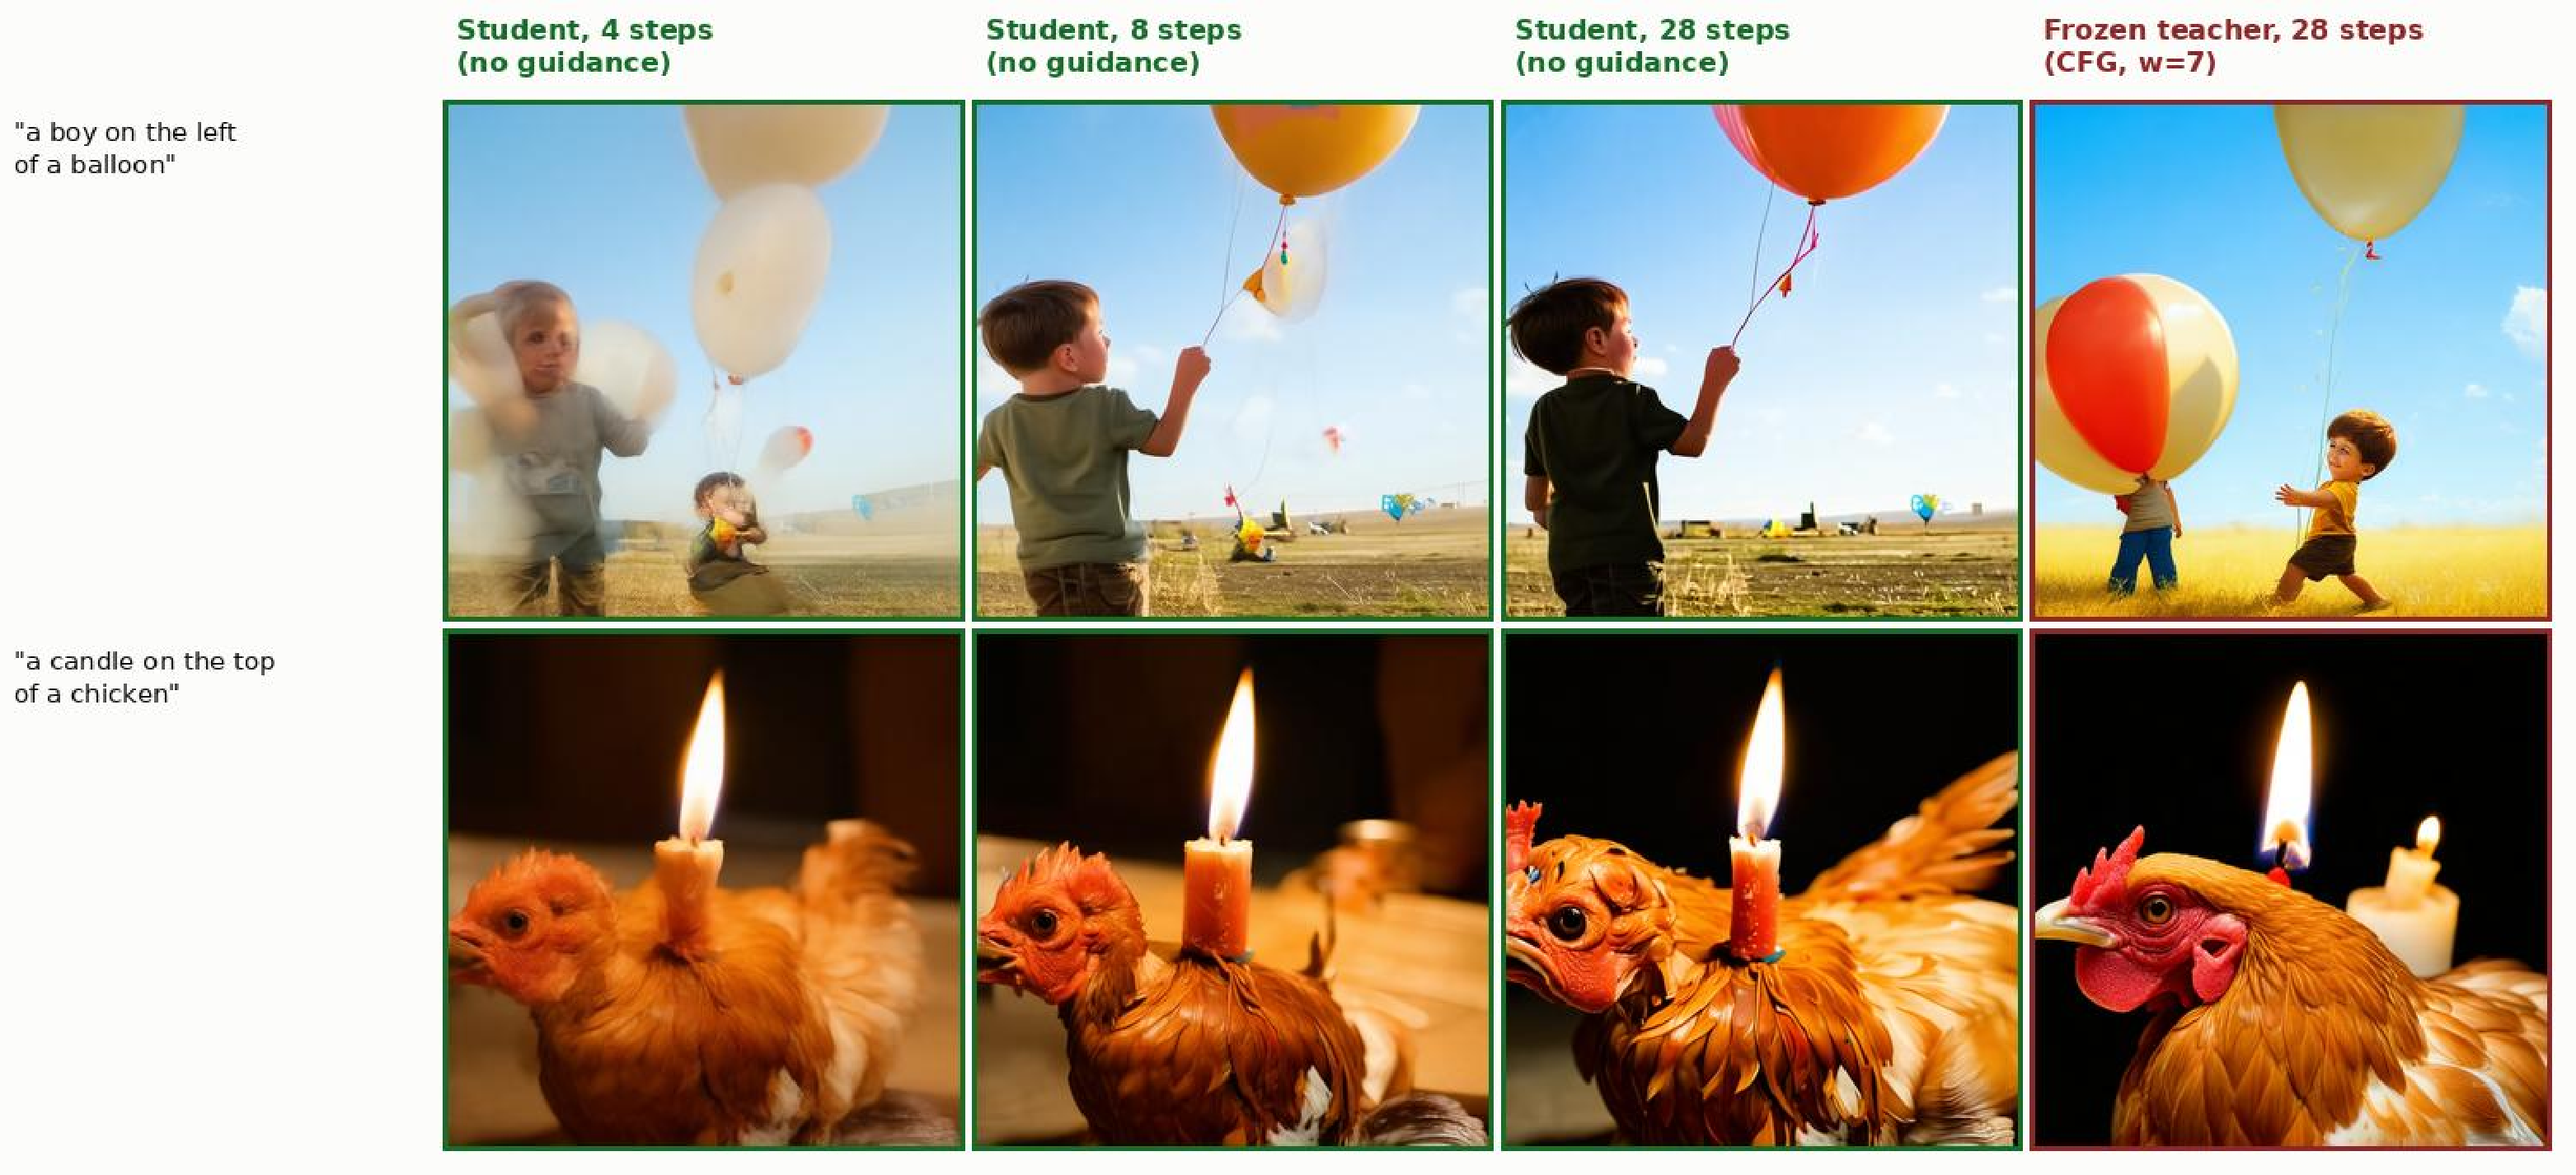
\includegraphics[width=0.95\textwidth]{qual_spatial_paper.pdf}
\caption{Two T2I-CompBench 2D-spatial prompts, identical initial noise per prompt (columns are not
independently seeded). Our student (argmax selection + projector reward, no guidance) places both
named objects in the requested relation at 4, 8 and 28 sampling steps alike; the frozen teacher with
guidance ($w{=}7$) does not, at 28 steps. Green borders: the requested relation is satisfied. Red
border: it is not. Automatic CompBench 2D-spatial scores (only computed for the trained 4-step
student and the teacher): 0.92 vs.\ 0.00 (top row), 0.78 vs.\ 0.00 (bottom row).}
\label{fig:qual}
\end{figure}

\section{Additional Ablations}
\label{sec:appendix-titles}
The following ablations were run on the 3k pool and are reported in full in the appendix; only
their titles are given here.
\begin{itemize}
\item Selection rule: argmax vs.\ Boltzmann-weighted vs.\ sampled vs.\ uniform candidate weighting.
\item Projector refresh schedule: frozen vs.\ refreshed every 100 updates at the default 4 steps vs.\
  16 steps (ours) vs.\ refreshed every 25 updates.
\item The decode-based reward's own reward-weight and rewarded-state sweep, as the point of
  comparison for Section~\ref{sec:results-train} (that sweep was run for the decode-based reward, not
  the projector, which was never tuned past the refresh schedule above).
\item Consistency-target horizon: 1-step Tweedie estimate vs.\ a 2-step chord vs.\ the trajectory endpoint.
\item Training objective: $x_0$ regression vs.\ segment-velocity imitation.
\item Teacher quality: candidate generation and training with a 16-step and a 28-step teacher.
\item Regression onto the reference photograph as a second training target.
\item An evolving (exponential-moving-average) teacher in place of the frozen teacher.
\item Number of candidates ($N{=}4$ vs.\ $N{=}8$) and optimiser batch size, at the 118k scale.
\item Inference step count: sampling the 4-step student at 2, 8, 16 and 28 steps.
\end{itemize}

\end{document}
